% JuliaCon proceedings template
\documentclass{juliacon}
\usepackage{amsmath}
\setcounter{page}{1}

\begin{document}

% **************GENERATED FILE, DO NOT EDIT**************

\title{Probabilistic Biostatistics with Julia}

\author[1]{Jeffrey A. Mills}
\author[1, 2]{Jeffrey R. Strawn}
\affil[1]{University of Cincinnati}
\affil[2]{Cincinnati Children's Hospital}

\keywords{Julia, Bayesian methods, Meta-analyses, Biostatistics, Randomized Controlled Trial}

\maketitle

\begin{abstract}

Medical research teams require statistical tools that are both sophisticated and powerful enough to address complex inferential problems, and also intuitive and user-friendly enough not to require advanced statistical and programming expertise.  Combining Julia with the Bayesian MCMC machinery can address this need; providing statistical tools that are powerful yet do not require the user to acquire advanced expertise in statistics or programming.
\vskip 6pt
Examples are given to illustrate the application of Bayesian probabilistic biostatistics in Julia, and include Bayesian adaptive trial design and sequential analysis of data from the CAMS randomized controlled trial of anxiety in youth, and Bayesian hierarchical modeling for a meta-analysis comparing the efficacy of different treatment side effects for adolescent anxiety.  The examples demonstrate that this combining Julia and Bayesian methods provides a sophisticatedly simple approach to statistical analysis and modeling for medical research.

\end{abstract}

\section{Introduction}

We know that Julia solves the “two-language problem”: it is both fast and efficient (performance), and easy to use (user friendliness).\cite{bezanson2017julia}  Using Julia combined with the Bayesian MCMC machinery can solve what we call “the two field problem”: that clinical researchers often need expertise in both the clinical field of their research topic and in statistical computing.  
\vskip 6pt
As those conducting and funding clinical randomized controlled trials (RCTs) recognize the high costs of these studies (e.g., medication expense, time required, and potential exposure of patients to ineffective treatments), there has been greater enthusiasm for (1) improving statistical analytic methods for RCTs, and 2) using evidence-based methods to examine existing naturalistically collected clinical data to inform clinical practice without the need for RCTs.  These approaches require far greater statistical and programming knowledge and sophistication from users.  Thus, there is an urgent need to provide statistical tools to clinician-researchers that are intuitive and easy to use, yet sophisticated and powerful enough “under the hood” to answer questions that simpler methods cannot.
\vskip 6pt
The “Bayesian machinery” of posterior simulation and Markov chain Monte Carlo (MCMC) methods together with Julia offer a solution to this “two-field problem”. This enables exact small sample inference and hypothesis testing for complex models without requiring the restrictive assumptions necessary to obtain analytical tractability (performance), and facilitates the analysis of complex models with basic statistical concepts: frequency distributions, density plots, means, medians, modes, standard deviations, quantiles, and posterior odds (user friendliness).\cite{Mills2019} 
\vskip 6pt
This paper presents some examples from our research developing and applying a Bayesian probabilistic approach to inference and testing in RCTs.\cite{Mills2019, Strawn2019, Strawn2018, Strawn2017, Strawn2018a} Our approach makes extensive use of posterior simulation and MCMC methods which, being recursive, require efficient looping to code effectively, so most available R packages rely on C++ code.  This leads to the two-language problem: either you have to code in C++ or something similar, or rely on a black box package.  Julia offers a pleasant and clean coding experience and many packages that, being written in Julia, allow one to examine and learn from the source code.  We are currently developing our own package, BayesTesting.jl,\cite{Mills2018} along with taking advantage of several Julia packages (e.g. Distributions.jl, DataFrames.jl, CSV.jl and Turing.jl) to apply MCMC and hierarchical models to conduct analyses and meta-analyses of data from RCTs.\cite{Strawn2019}

\section{Moving Hypothesis Testing Forward}
\label{sec:hypothesistest}

\begin{quote}
	At some future time trials may be evaluated using fully Bayesian notions of utilities and decisions ... which would enable designs to be built that do not violate the Likelihood Principle or Bayesian notions.  But currently, the regulatory structure is such that confirmatory trials are usually judged and evaluated using Type I error.\cite{Berry20ll}, p.220-221.
\end{quote}
\vskip 6pt
Despite widespread and persistent criticism of p-values,\cite{Berry2017} the ``$p \le 0.05$ is ‘statistically significant’, $p > 0.05$ is not'' is an iron law for publishing in leading journals in many fields. In general, you cannot successfully publish applied science without precise hypothesis testing.  Statisticians, especially Bayesians, argue against that approach, but there is far too much institutional inertia and bias towards precise testing and use of $p$-values as `proper’ applied science.  At the very least, we need a bridge from `pure’ hypothesis testing to a more complete Bayesian analysis.
\vskip 6pt
The comparison of means from two samples provides a canonical example. Suppose we have samples from two different treatments, $x_1$ and $x_2$ and wish to evaluate the evidence on whether there is any difference in average treatment effect (ATE).  This is equivalent to evaluating the precise vs. composite hypotheses,  
\begin{equation} 
H_0: \delta = 0, \; \; H_1: \delta \ne 0. 
\label{eq:hoh1}
\end{equation}
where $\delta = \mu_1 - \mu_2$, and $\mu_j$ is the ATE for treatment $j$.

Appealing to the Central Limit Theorem and the Principle of Maximum Entropy provides strong justification for assuming that the distribution of the sample mean, $\bar{x}_j$, for each sample (i.e. the likelihood) is Gaussian, 
\begin{equation}
\bar{x}_j \sim N(\mu_j,\sigma_j^2/n_j ), \; \;    j=1,2,
\label{eq:xbar}
\end{equation}
where $\sigma_j^2$ is the variance of $x_j$ and $n_j$ is the number of observations in sample $x_j$. Adopting uninformative priors for the mean and variance leads to conditional posterior densities,
\begin{equation}
\mu_j | \sigma_j,x_j \sim N(\bar{x}_j, s_j^2),
\label{eq:muj}
\end{equation}
\begin{equation}
\sigma_j^2|\mu_j,x_j \sim IG((n_j-1)/2,(n_js_j^2)/2).
\label{eq:sigmaj}
\end{equation}
where $s_j^2$ is the sample variance. This is as far as we need to go analytically.  The rest of the problem can be solved numerically.
\vskip 6pt
Obtaining $M$ draws from these conditional distributions provides pseudo-samples from the marginal posteriors for $\mu$ and $\sigma^2$.  We then obtain an MCMC pseudo-sample of size $M$ from the posterior distribution of $\delta$, $\delta^{(m)} = \mu_1^{(m)} - \mu_2^{(m)},$ $m = 1,...,M$.  In this way, posteriors for any function of the parameters is available, such differences in differences and ratios. For example, we often wish to compare two treatments to placebo, then to each other, which is accomplished by obtaining $\Delta^{(m)} = \delta_1^{(m)} - \delta_2^{(m)}$. While the analytical distribution of $\Delta$ is unknown and asymptotic approximations require unrealistic assumptions,  MCMC sampling allows the exact small sample posterior density to be approximated arbitrarily closely as $M$ is increased. The rest of the analysis requires only knowledge of basic statistics: plotting the density of the MCMC draws, computing summary statistics, and testing hypotheses.   Note that this addresses the Behrens-Fisher problem, allows for different unknown variances in each sample, and allows for different sample sizes.  Correlation across samples and other model extensions are straightforward.
\vskip 6pt
To test the hypotheses in (\ref{eq:hoh1}) we evaluate the posterior odds against $H_0$,$ O(\delta = 0)$, by evaluating the MCMC posterior density for $\delta$ at the value in the null hypothesis, $0$, and at the mode,
\begin{equation}
O(\delta = 0|x_1, x_2) = \frac{p(\delta=\delta_{MAP}|x_1,x_2)}{p(\delta=0|x_1,x_2)},
\label{eq:odds}
\end{equation}
where $\delta_{MAP}$ is the maximum a posteriori estimate of $\delta$.
We can also compute a one-sided Bayesian p-values from the MCMC sample,
\begin{equation}
p(\delta \le 0|x_1, x_2) =  \frac{\sum_{m=1}^M I_m }  {M},
\label{eq:pval}
\end{equation}
where $I_m = 1$ if  $\delta^{(m)} \le 0$, $0$ otherwise.  These same formulas can be used to evaluate hypotheses concerning other quantities of interest, such as $\Delta$.

\section{Bayesian adaptive trial design and sequential analysis}
Bayesian adaptive trial design and sequential analysis of data from an RCT can be accomplished using the Bayesian machinery outlined above. An advantage of the Bayesian approach in this context as that it involves no statistical requirement for a stopping rule.  Though other reasons for a stopping rule are important, such as funding and avoiding bias due to stopping when a test critical value is reached, a sequential analysis can minimize costs, time and the number of subjects exposed to inferior treatment.  Further, there is no satisfactory frequentist differences of differences analysis without restrictive assumptions – the analytical distributions are not known and not tractable, asymptotic assumptions are not valid since we are often dealing with small samples and there may be other constraints (such as boundary conditions). Bootstrapping is also inferior due to the small sample sizes (‘a poor person’s MCMC’). The commonly used Welch t-test is an ad hoc attempt to deal with different variances across samples that does not perform well in simulations.\cite{Mills2019}  All of these issues are resolved by using the Bayesian MCMC machinery.
\vskip 6pt
In previous work,\cite{Strawn2018,Mills2019} categorical and quantitative outcome data from a federally-funded NIH trial of pediatric patients with anxiety disorders (Child/Adolescent Anxiety Multimodal Study [CAMS], N=488) were analyzed to validate the proposed methodology and examine treatment and placebo responses in this RCT. CAMS included patients aged 7-17 years of age (mean age: 10.7 years) who met DSM-IV criteria for >1 pediatric anxiety triad disorders (GAD, SAD or social anxiety disorder/social phobia). Those included in the trial were randomized (2:2:2:1) to the following: cognitive behavioral therapy (CBT, n=139), the SSRI sertraline (SRT, n=133), SRT+CBT (n=140), or pill placebo (PBO, n=76).
\vskip 6pt
The following example sequantially analyze the data for the combined treatment SRT+CBT relative to PBO using Bayesian updating.  We wish to evaluate the hypothesis in equation~(\ref{eq:hoh1}) where $\mu_1$ is the average treatment effect (ATE) of Sertraline+CBT and $\mu_2$ is the ATE of the placebo. Starting with a sample of 12 (8 treated, 4 placebo), the posterior density was updated with each additional 6 observations (4 treated:2 placebo).  The sequence of posteriors as $n$ is increased for the difference in ATE between the SRT+CBT and placebo groups is illustrated in Figure \ref{fig:pars_diff}.
% insert pars_difference_sequential.png
\begin{figure}[t]
	\centerline{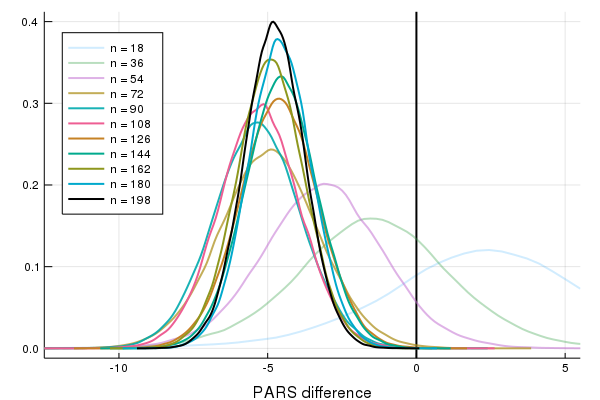
\includegraphics[width=8cm]{pars_difference_sequential.png}}
	\caption{Difference in ATE between treatment and placebo groups.} 
	\label{fig:pars_diff}
\end{figure}

\begin{figure*}[t]
	\centerline{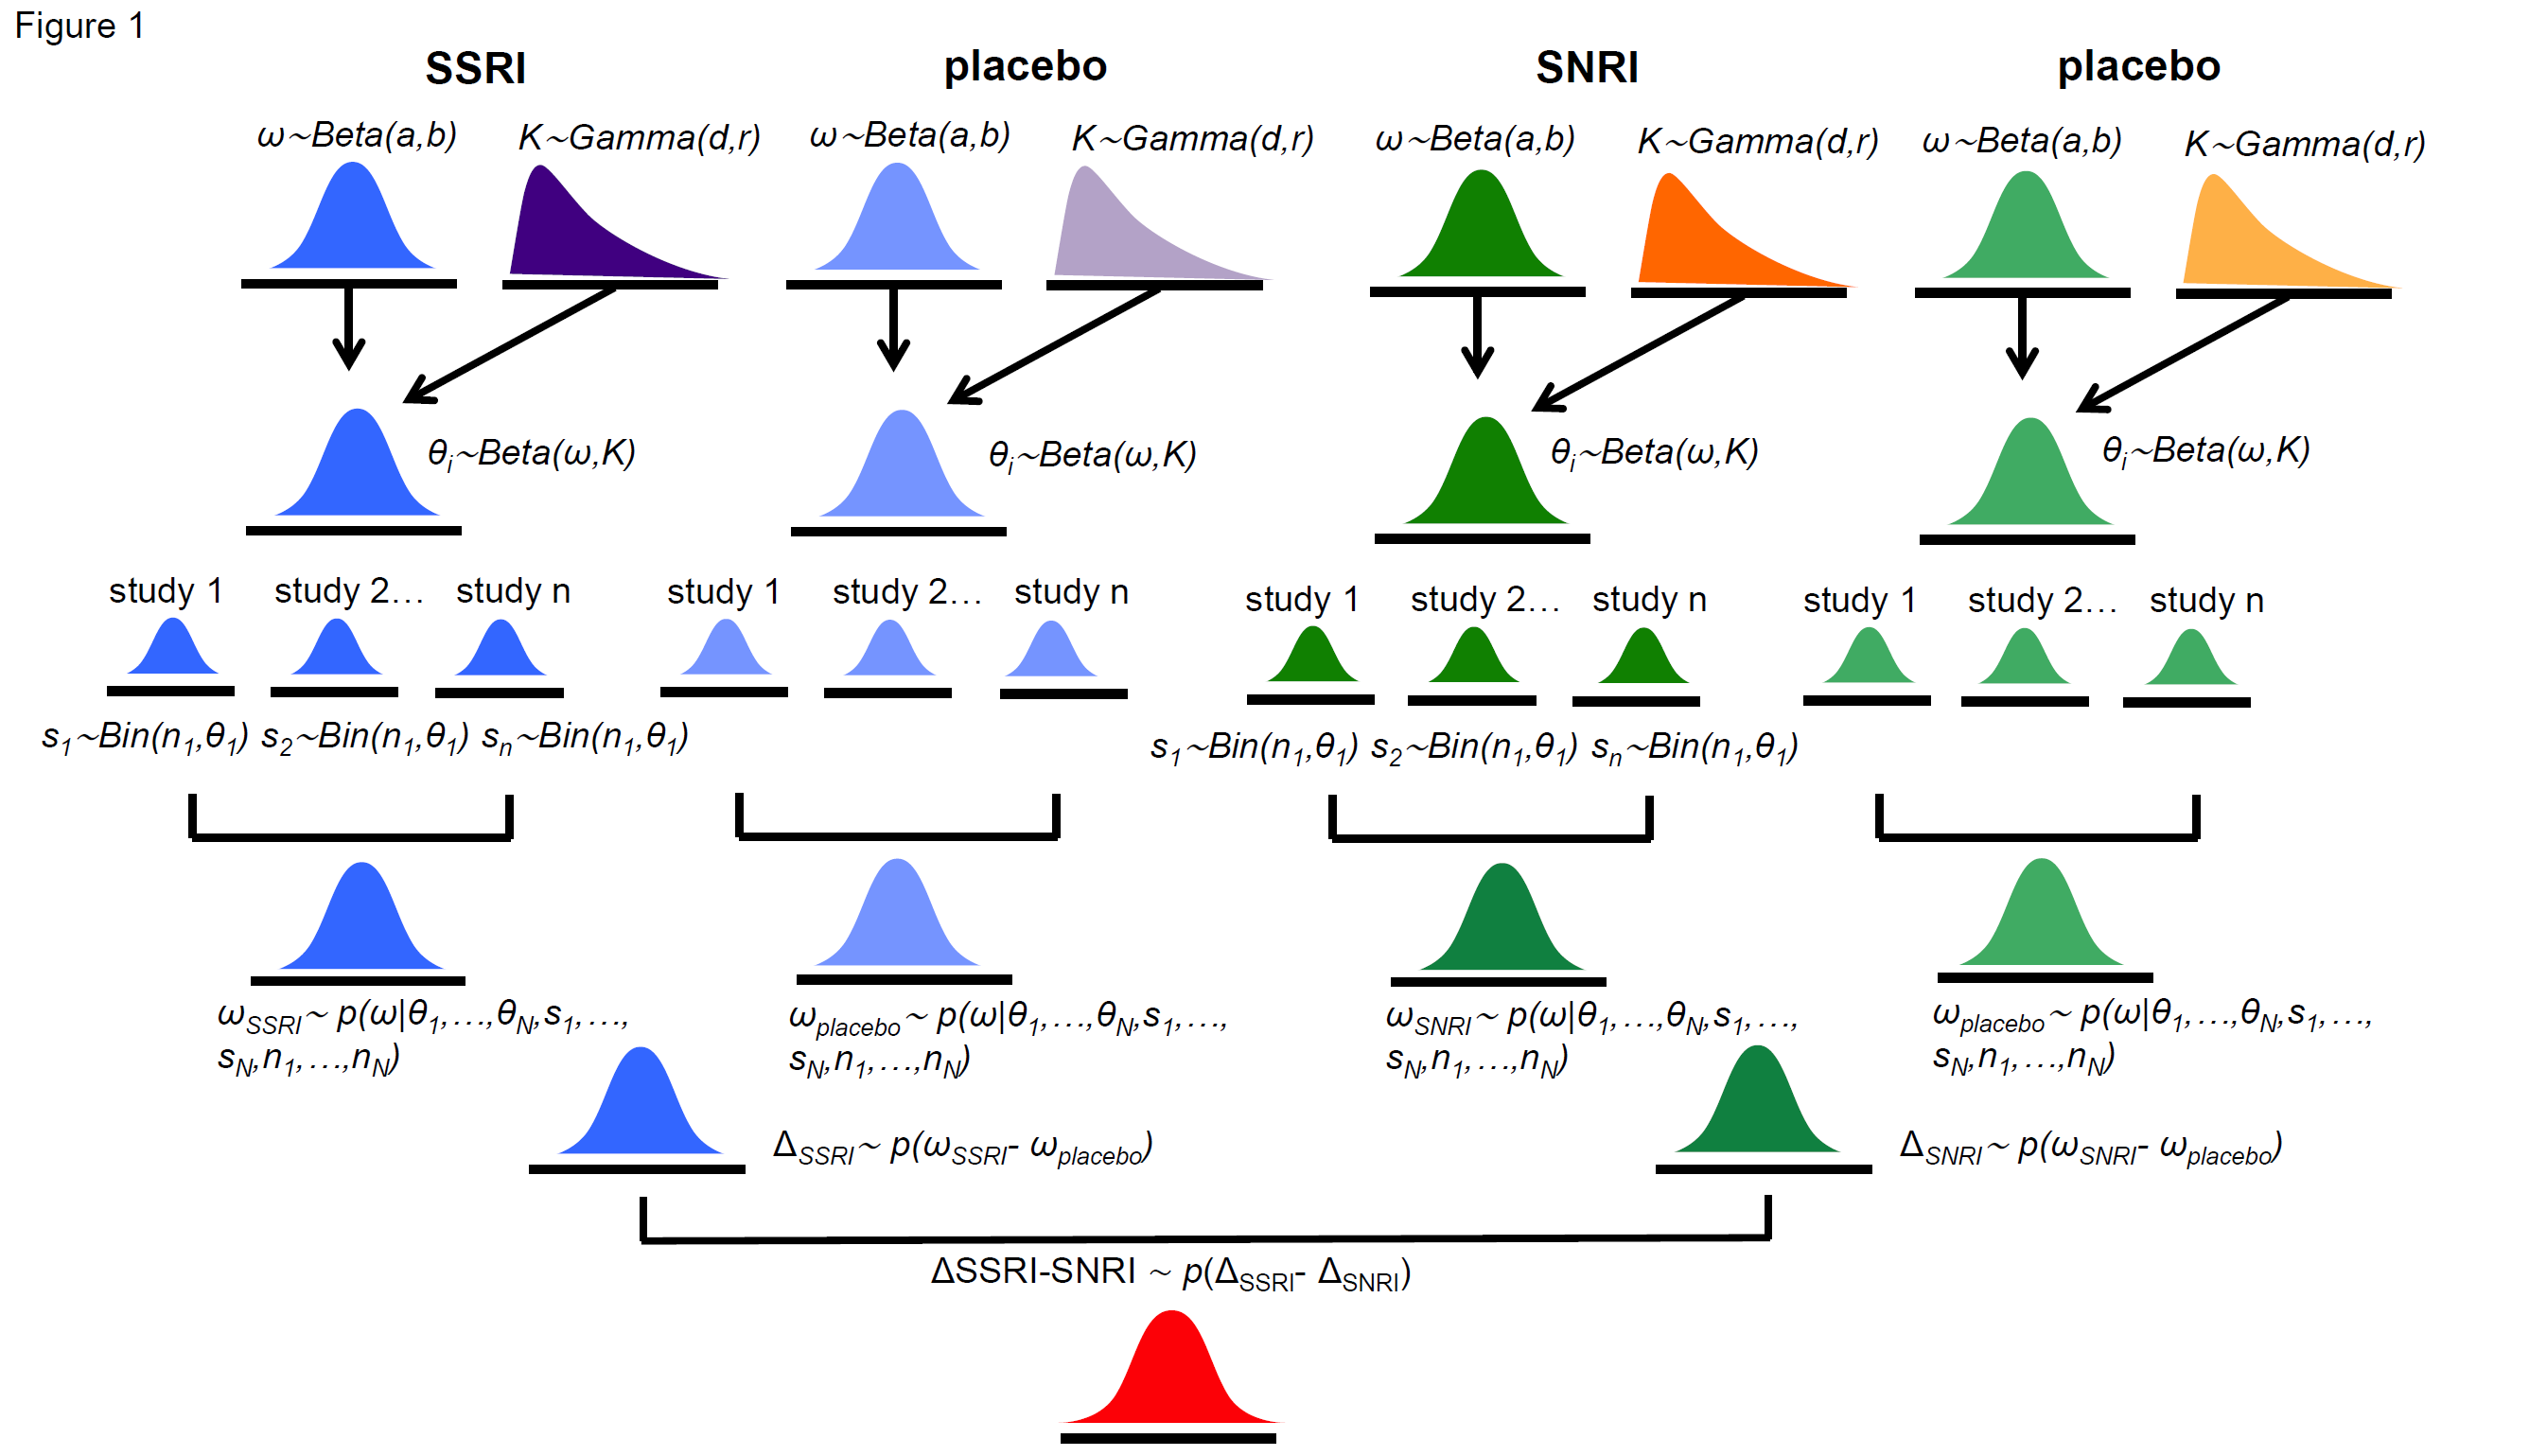
\includegraphics[width=18cm]{bhm_model.png}}
	\caption{Bayesian Hierarchical Model for Treatment Comparisons.}
	\label{fig:bhm}
\end{figure*}
\vskip 6pt
There is clear evidence of a difference in efficacy between the SRT+CBT treatment and PBO, $\delta$, by $n=72$ (posterior odds against $H_0:\delta=0.0$ are $70.4$:$1$, $p(\delta \ge 0|s,n) = 0.002$,), suggesting that the CAMS study could have been completed with less than half of the original sample with no change in the categorical or quantitative outcome conclusions.


\section{Bayesian hierarchical modeling}
\label{sec:hbm}
A Bayesian hierarchical model (BHM) provides a flexible setting for modeling categorical data that allows for heterogeneity across individuals or groups. If homogeneity across studies is assumed, the data can be combined via Bayesian updating as in the sequential analysis in the previous section.  All that is needed are the number of occurrences, $s_i$, in $n_i$ subjects in each study, $i$, of $N$ studies.  he posterior distribution is then 
\begin{equation}
\begin{split}
p(\theta | s_1,...,s_N, n_1,...,n_N,a,b) = \\ \textnormal{Beta}(\sum_{i=1}^N (s_i +a),\sum_{i=1}^N(n_i - s_i) + b),
\end{split}
\label{eq:pbeta}
\end{equation}
with $a=b=1$ for a uniform prior for $\theta$.
\vskip 6pt
Alternatively, BHM can be specified to allow for heterogeneity across studies due to different trial sites, different types of treatment, such as different families of anxiety medication (SSRI or SNRI), etc., and the same Bayesian machinery can be employed to compare a variety of treatments relative to placebo. For the categorical data examined herein there are two common BHM specifications: the Beta-Gamma,\cite{Kruschke2014} and the logistic-normal.\cite{Mcelreath2015}.  In the following, we adopted the Beta-Gamma BHM specification as it directly provides intuitively understandable parameter estimates, whereas the logistic specification is more difficult to interpret.
\vskip 6pt
The complete BHM Beta-Gamma modeling framework is illustrated in Figure \ref{fig:bhm} for the case of comparing two sets of RCTs for different treatments (SSRI vs. SNRI) with placebo groups in each RCT. Each study in Figure \ref{fig:bhm} has a Binomial likelihood for $s$ successes in $n$ trials with probability of success $\theta$ (row 3).  A Beta prior with mode $\omega$ and precision parameter $K$ is assigned to each $\theta$ (row 2), and a Beta and Gamma hierarchical prior are assigned to $\omega$ and $K$ respectively (row 1). The hyperparameters $a,b,d$ and $r$ are selected to represent a priori knowledge about the distribution of each $\theta$ (typically relatively uninformative priors are assigned unless other information is available).
\vskip 6pt
The package Turing.jl provides HMC and MCMC algorithms to obtain posterior density MCMC chains from an essentially unlimited variety of models through Julia macros that provide a flexible and intuitive modeling and inference framework. The model specification in Turing.jl closely matches how one would write the model mathematically (Turing code examples for the logistic-normal are available at github.com/TuringLang/Turing.jl and github.com/StatisticalRethinkingJulia):
\begin{lstlisting}[language = Julia]
# Turing.jl BHM for binomial trials
using Turing, MCMCChains
@model binomial_trials(s,n) = begin
g = length(n)  # number of groups
# hierarchical priors
w ~ Beta(2,3)
KappaMinusTwo ~ Gamma(10,1/0.05) 
a = w*KappaMinusTwo + 1.0
b = (1.0 - w)*KappaMinusTwo+1.0
# priors for each occurrence rate
theta = Array{Real}(undef, g)
for k in 1:g
theta[k] ~ Beta(a,b)
end
# likelihood
for i in 1:g
s[i] ~ Binomial(n[i],theta[i])
end
end;
\end{lstlisting}

Only a few more lines of code are need to obtain posterior samples from the No U-Turn Hamiltonian Monte Carlo sampler in Turing.jl and then examine the posterior and test the hypothesis of no difference in side effect occurrence between two groups:
\begin{lstlisting}[language = Julia]
using BayesTesting

# treatment
ct = mapreduce(c->sample(binomial_trials(s2, n2),  
NUTS(5000,1000,0.65)),chainscat,  1:5)

# placebo
cp = mapreduce(c->sample(binomial_trials(s1, n1), 
NUTS(5000,1000,0.65)), chainscat,  1:3)

wt_draws = Array(ct["w"][1001:end])  # treatment w
wt_draws = Array(ct["w"][1001:end])  # placebo w
diff = wt_draws - wp_draws           # difference
plot(diff,st=:density,label="Difference")

# compute mean, SD, odds and tail prob.
[mean(diff) std(diff)]
quantile(diff,[0.025,0.5,0.975])
[mcodds(diff, h0=0.0) bayespval(diff)]
\end{lstlisting}

In recent work,\cite{Mills2019b} a meta-analysis of results from several different RCTs was conducted to obtain more complete evidence on the expected side effects of SSRIs.  Side effect or adverse event (AE) occurrence in an RCT is generally recorded as a categorical variable, leading to binomial data consisting of number of Aes, $s_j$, in $n_j$ subjects for trial $j$. The results below are for the  “activation” (or restlessness) AE.  Five studies included data for activation.  Posteriors for each of the five studies for treatment (with SSRI) and placebo were obtained using Turing.jl (the third row of distributions in the \ref{fig:bhm}), along with the distribution of the mode, $\omega$, of the posterior for the estimated rate of success for each study, $\theta_i$ (the fourth row in the Figure \ref{fig:bhm}).  Given the MCMC pseduo-samples for each $\omega$ (side effect response to SSRI and response to placebo), differences in treatment to placebo, then differences in differences between the two treatments relative to placebo can be computed (rows 5 and 6 in the Figure \ref{fig:bhm}).
\vskip 6pt

Using the No U-Turn Hamiltonian Monte Carlo sampler in Turing.jl, the BHM is estimated for each treatment arm of the study data. The stability of the chains suggests convergence to the marginal posteriors has been attained, as illustrated in Figure \ref{fig:chains}.
\begin{figure}[t]
	\centerline{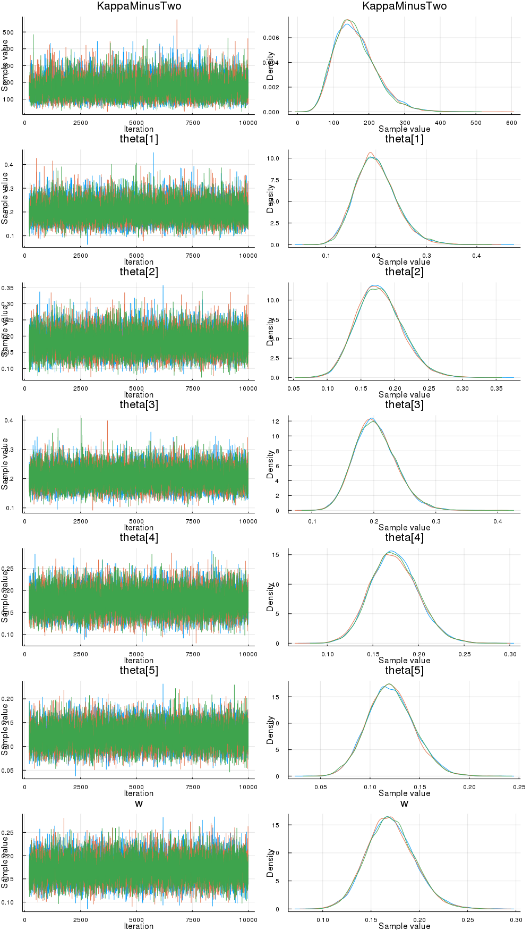
\includegraphics[width=8cm]{mc_chains.png}}
	\caption{HMC chains from No U-Turn Sampler.}
	\label{fig:chains}
	\end{figure}

The resulting posterior densities for each study probability of occurrence rate (risk), $\theta_j$ and the hierarchical probability of occurrence across groups, $\omega$ are illustrated in Figure \ref{fig:activ}. Results using the logistic-normal specification gave very similar results. The results for activation SERT+CBT (mean difference between treatment and placebo $\omega$ = 2.39, $p(\omega \ge 0|s,n) = 0.0015$, posterior odds against no difference $= 122.3$:$1$) provide statistical evidence of an increased likelihood of activation with the treatment. To examine the impact of across study heterogeneity, Figure \ref{fig:compare} presents the BHM posterior density for $\omega$ in comparison to combining all studies ignoring across study heterogeneity via equation~(\ref{eq:pbeta}).

\begin{figure}[t]
	\centerline{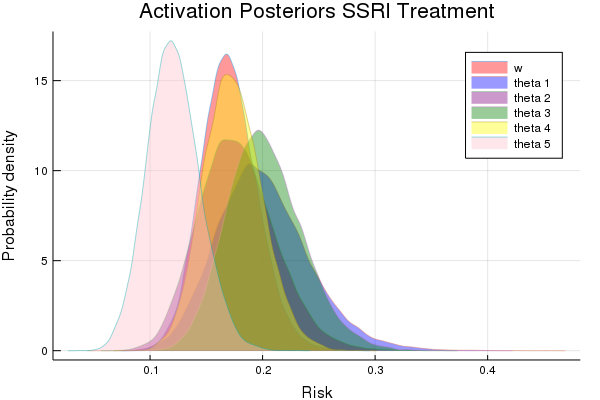
\includegraphics[width=8cm]{activation_posteriors.png}}
	\caption{Posterior Densities for Activation}
	\label{fig:activ}
\end{figure}

\begin{figure}[t]
	\centerline{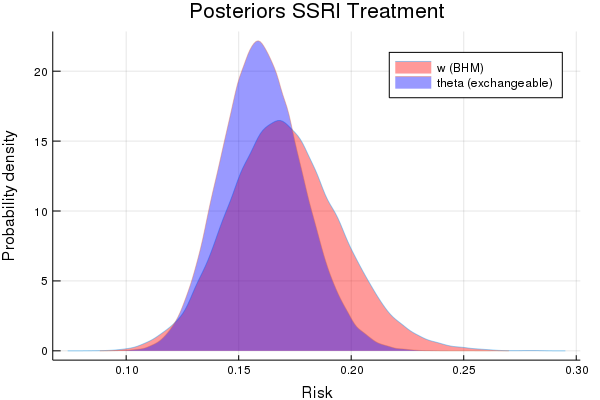
\includegraphics[width=8cm]{bhm_vs_non_compare.png}}
	\caption{ATE posterior density with and without heterogeneity}
	\label{fig:compare}
\end{figure}
 
\section{Summary and Conclusions}
This paper presented two examples of application of Bayesian probabilistic modeling from our own research that illustrate our experiences with Bayesian inferential methods for clinical research using Julia.  We have used this approach in several studies including: Reevaluating the evidence from previously conducted RCTs; analysis of abandoned trials; joint evaluation of tolerability and efficacy in RCTs; and Bayesian hierarchical modeling for meta-analysis evaluating adverse events (“side effects”) in trial participants.
\vskip 6pt
The approach presented provides a solution to the strong institutional bias/inertia of `$\le 5\% =$ statistical significant’ through provision of posterior odds as well as posterior tail probabilities (`Bayesian p-values’), posterior density intervals, and visualization of posterior densities. This further allows for more flexibility in the choice of critical value for a particular test, i.e. the cut-off point for rejecting vs. failing to reject the null hypothesis.  For example, researchers at CERN attempting to detect gravitational waves would wish to employ a much larger critical odds ratio (akin to the `5-sigma rule'), whereas researchers comparing the efficacy of two relatively harmless psychiatric treatments for anxiety or depression would undoubtedly find posterior odds that pass a much lower critical threshold convincing enough to recommend one treatment over another.  
\vskip 6pt
One of the major advantages of the contemporaneous Bayesian approach is 
the ability to utilize MC and MCMC computational methods. This approach is computationally very intensive but far less mathematically and analytically burdensome, and typically requiring far fewer restrictions than needed for analytical tractability.  Further, we find Julia to be  perfect for scientific programming of this nature, greatly reducing the burden on the researcher to wear multiple expertise `hats'. The resulting conservation of time and energy of the applied researcher from using Julia is substantial, allowing greater focus on the substantive scientific problem.

%\bibliographystyle{juliacon}
%\bibliography{ref}
%\end{verbatim}
%When submitting the document source (.tex) file to external
%parties, the ref.bib file should be sent with it.
%\cite{bezanson2017julia}

% **************GENERATED FILE, DO NOT EDIT**************

\bibliographystyle{juliacon}
\bibliography{ref.bib}

\end{document}

% Inspired by the International Journal of Computer Applications template